\chapter{Proposta de solução}
\label{cap:propostadesolucao}

Neste capítulo será proposto uma solução de implementação de um ambiente de alta disponibilidade para os serviços críticos da empresa, que 
foram selecionados no capítulo anterior. Com isso pretende-se atingir o objetivo deste trabalho.

O primeiro passo desta implementação é fazer uma reorganização das máquinas virtuais entre os servidores atuais, liberando assim o 
\textit{hardware} suficiente para possibilitar a implementação do ambiente de alta disponibilidade. 

Após ter sido feito a reorganização das máquinas virtuais será iniciado a implementação, montando um ambiente com dois servidores e os 
configurando de uma forma que caso houver alguma falha, em um servidor físico ou no seu sistema operacional hospedeiro, as máquinas serão 
tranferidas para o outro servidor físico. 
A configuração deverá ser: 11 \textit{cores} de processamento, 12 GB de memória e 156 GB de disco para cada servidor. Essa configuração foi 
calculada a partir da soma dos recursos atuais das máquinas virtuais que possuem os serviços críticos, que foram apresentadas no capítulo
anterior na Seção \ref{section:servcrit}.

As ferramentas necessárias para essa implementação podem ser divididas em dois tipos: ferramenta de replicação de dados 
(Seção \ref{section:toolrepl}) e ferramenta que faz o monitoramento e a tranferências das máquinas virtuais em caso de falhas 
(Seção \ref{section:toolcluster}).

\section{Ferramentas de replicação de dados}
\label{section:toolrepl}

Replicação de dados pode ser feita de diversas maneiras, pode ser a nível de aplicação ou até mesmo a nível de \textit{hardware}.
Dependendo do objetivo e da aplicação pode-se usar ferramentas como por exemplo o \textit{rsync}, que faz o sincronismo de dados de uma origem
para um destino. Sendo assim, não é possível utilizar essa ferramenta, pois ela não faz a replicação em tempo real, ou seja, se for necessário
utilizar os dados de destino ocorrerá perda de dados. Outra forma de replicação é a de discos com \ac{RAID} por exemplo, essa solução é eficaz
para garantir que o sistema não fique indisponível em caso de falha de discos\footnote{Lembrando que essa solução é utilizada no ambiente atual
para aumentar a disponibilidade dos servidores}, porém não garante a disponibilidade quando algum componente de \textit{hardware} falhar 
\cite{zaminhani2008}.

A solução de replicação ideal para esta implementação é um espelhamento de dados através da redes, assim permitindo a cópia dos dados para uma
máquina remota. Essa solução além de fazer a replicação dos dados, faz a redundância de todo \textit{hardware}.

A ferramenta escolhida para replicação de dados na solução de alta disponibilidade desse trabalho foi o \ac{DRBD}. Essa ferramenta é de código
aberto, e permite a replicação de dados de um dispositivo local em tempo real. 
APROFUNDAR AQUI OU NA IMPLEMENTAÇÂO?

% dispositivo primario e secundario zaminhani2008
% Segundo (ELLENBERG, 2007), a partir da versão 8 do DRBD é possível que,
%dependendo da aplicação, a execução ocorra em todos os nós do cluster
%simultaneamente (Ativo/Ativo). Para tornar isso possível é necessária a
%utilização de um sistema de arquivos exclusivo para cluster, como o OCFS2 6 e o
%GFS 7 por exemplo. Como a abordagem deste trabalho é cluster de alta
%disponibilidade, a utilização do DRBD no modo Ativo/Ativo não será discutida.

\section{Ferramentas de gerenciamento de cluster?}
\label{section:toolcluster}

Para ser possível implementar uma solução de alta disponibilidade é necessário uma ferramenta que monitora os recursos, fazendo a detecção e
recuperação do serviço utilizando mensagens entre os servidores \cite{perkov2011}.

\textit{Pacemaker} é uma ferramenta de detecção e recuperação de falhas a nível de serviço \cite{perkov2011}. Essa ferramenta é um projeto da
xx, ele é classificado como um CRM...
Continuar ??? \textit{Heartbeat} ou \textit{Corosync} \cite{zaminhani2008}.

cluster resource manager (CRM) which has the task of starting and stopping the services (IP addresses, web servers, etc)
 
live migration \ref{fig:vms_migration}
%http://www.aliancatecnologia.com/conteudo/2015/05/quatro-estrategias-de-protecao-para-seu-ambiente-virtual/

\begin{figure}[h!]
 \centering
 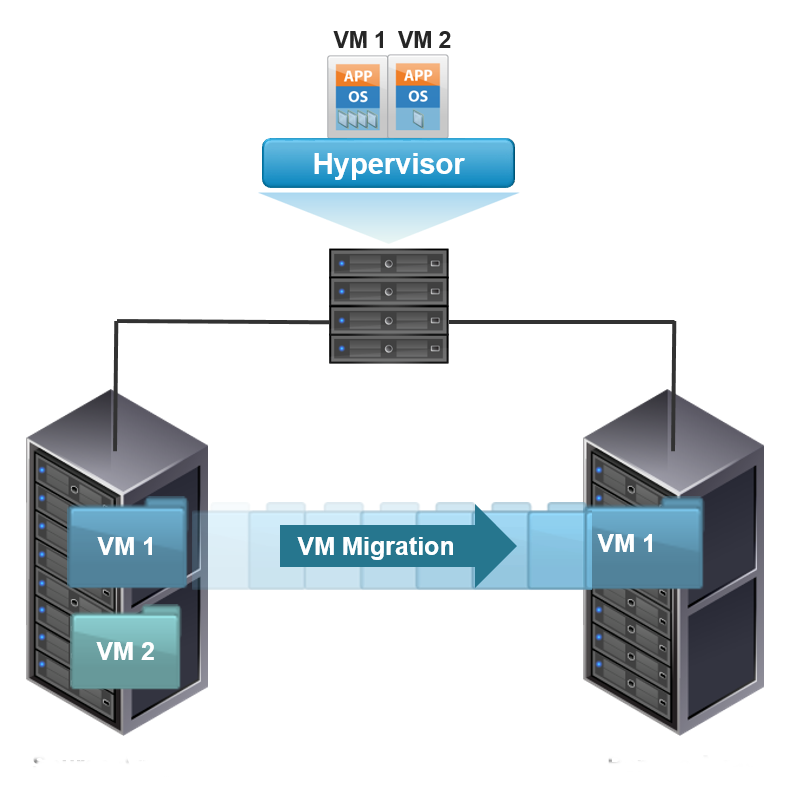
\includegraphics[width=300px]{img/vms_migration.eps}
 \caption{Live migration}
 Fonte: \citet{spaniol2015}
 \label{fig:vms_migration}
\end{figure}


%reorganização de vms
%ferramentas selecionadas, colocar motivo para escolher e citar ferramentas parecidas
%muitos servicos, melhor solucao utilizar 2 servidores para fazer redundancia
%em caso de falha de um servidor fisico...
%ferramentas open source...
%colocar a disponibilidade do nagios do ano passado?
